\documentclass[10pt,a4paper]{beamer}
\usepackage[utf8]{inputenc}
\usepackage[english,bulgarian]{babel}
\usepackage{amsmath, amsfonts, amssymb, amsthm, bigints, textcomp, caption, subcaption, float, graphicx, tikz, xcolor}
\usetikzlibrary{arrows,shapes,positioning}
\newcommand\ytl[2]{
    \parbox[b]{8em}{\hfill{\color{cyan}\bfseries\sffamily #1}~$\cdots\cdots$~}\makebox[0pt][c]{$\bullet$}\vrule\quad \parbox[c]{4.5cm}{\vspace{7pt}\color{red!40!black!80}\raggedright\sffamily #2.\\[7pt]}\\[-3pt]
}

\usetheme{Madrid}

\title{ Скаларно тензорни теории - новата истина за гравитацията }
\author{ Димитър Попчев }
\institute{ Софийски Университет „Св. Климент Охридски“ }
\titlegraphic{ 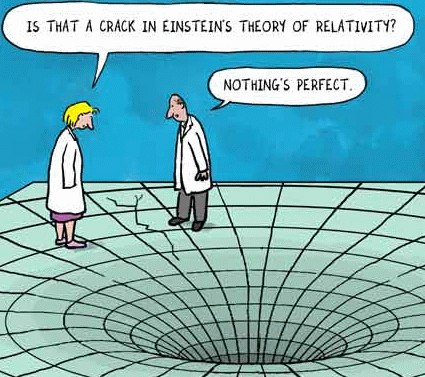
\includegraphics[scale=0.25]{images/GR_crack_intro.png} }

\newcommand*{\yellowemph}[1]{%
	\tikz[baseline]\node[rectangle, fill=yellow, rounded corners, inner sep=0.3mm,anchor=base]{#1};%
}

\begin{document}
	
	\begin{frame}
		\titlepage
	\end{frame}
	
	\section{ История }

		\begin{frame}{}
			\tableofcontents[currentsection]
		\end{frame}
		
		\begin{frame}{ Исторически бележки }
            \begin{table}
                \centering
                \begin{minipage}[t]{.7\linewidth}
                    \color{gray}
                    \rule{\linewidth}{1pt}
                    \ytl{$\sim$330 BCE}{Аристотелова механика}
                    \ytl{1589}{Галилеева механика}
                    \ytl{1687}{Нютонова механика}
                    \ytl{1859}{Аномалия на перихелия на Меркурий}
                    \ytl{1916}{Обща теория на относителността}
                    \ytl{1961}{Теория на Бранс-Дике}
                    \ytl{1979}{Скаларно-тензорни теории}
                    \bigskip
                    \rule{\linewidth}{1pt}%
                \end{minipage}%
            \end{table}
		\end{frame}
        
        \begin{frame}{ Аристотелова механика }
			\begin{columns}
				\begin{column}{0.6\textwidth}
					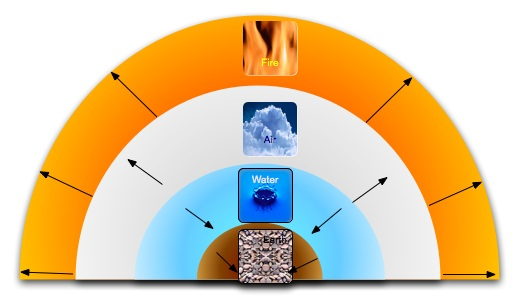
\includegraphics[width=\textwidth]{images/aristotle_four_elements_motion.jpg}
				\end{column}
				\begin{column}{0.4\textwidth}
					\begin{itemize}
						\item Четири основни елемента
                        \item Естествено движение
                        \item $ v \sim m $
                        \item $ v \sim 1/b $
					\end{itemize}
				\end{column}
			\end{columns}
        \end{frame}
		
        \begin{frame}{ Аристотелова механика }
            \begin{center}
                
                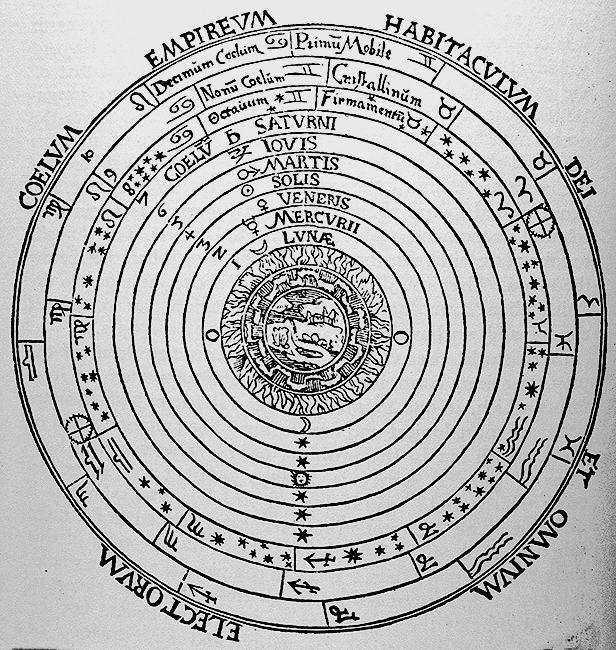
\includegraphics[scale=0.3]{images/aristotel_universe.png}
                
            \end{center}
        \end{frame}

        \begin{frame}{ Наследство на Аристотел }
            \begin{columns}
                \begin{column}{0.5\textwidth}
                    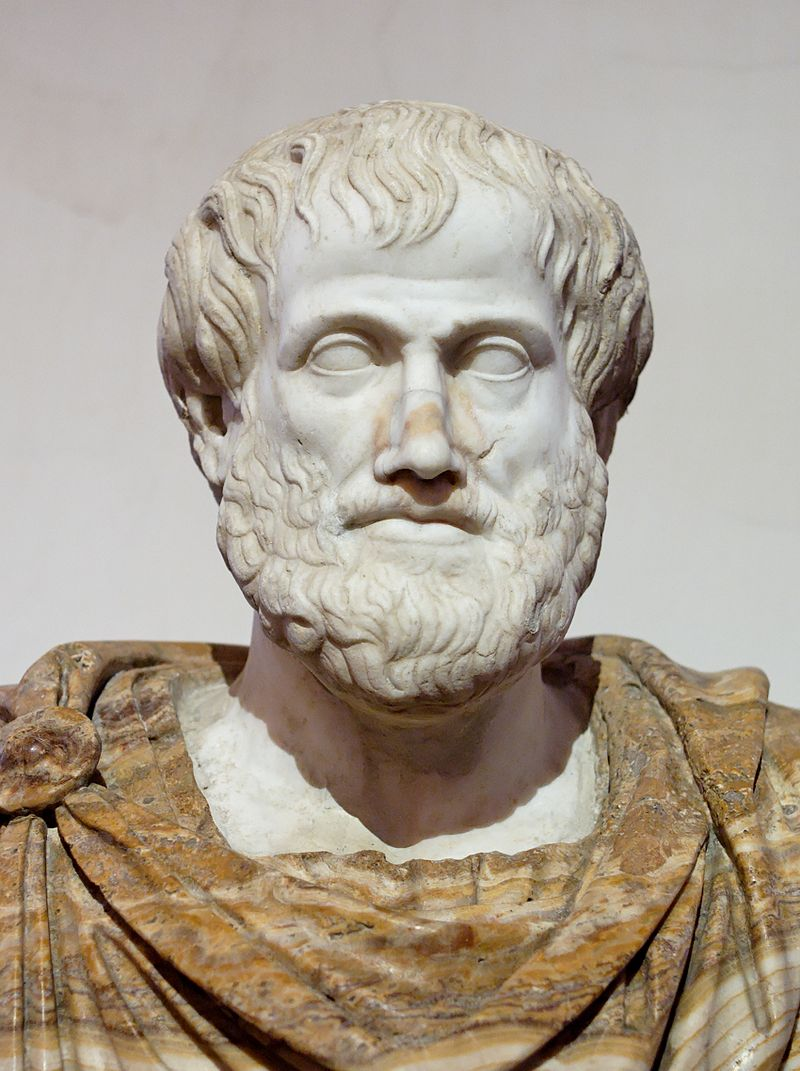
\includegraphics[width=0.9\textwidth]{images/aristotle_portrait.jpg}
                \end{column}
                \begin{column}{0.5\textwidth}
                    \begin{itemize}
                        \item Научно познание
                        \item Модел на Вселената
                    \end{itemize}
                \end{column}
            \end{columns}
        \end{frame}
    
        \begin{frame}{ Наследство на Аристотел }
            \begin{columns}
                \begin{column}{0.5\textwidth}
                    
\includegraphics[width=\textwidth]{images/aristotel_vs_galiele.png}
                \end{column}
                \begin{column}{0.5\textwidth}
                    \begin{itemize}
                        \item Научно познание
                        \item Модел на Вселената \\
                        \noindent\rule{5cm}{0.5pt}
                        \item ... до Галилей
                    \end{itemize}
                \end{column}
            \end{columns}
        \end{frame}
    
        \begin{frame}{ Галилеева механика }
            \begin{columns}
                \begin{column}{0.5\textwidth}
                    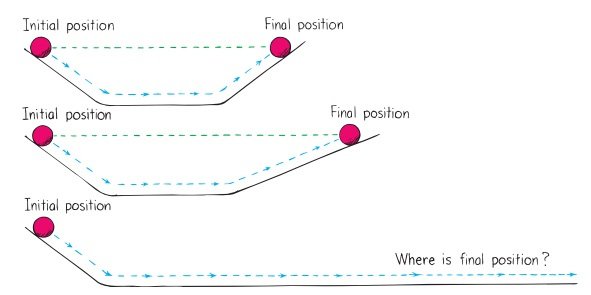
\includegraphics[width=\textwidth]{images/galilei_ramps.jpg}
                \end{column}
                \begin{column}{0.5\textwidth}
                    \begin{itemize}
                        \item Експерименти с рампи
                    \end{itemize}
                \end{column}
            \end{columns}
        \end{frame}
    
        \begin{frame}{ Галилеева механика }
            \begin{columns}
                \begin{column}{0.5\textwidth}
                    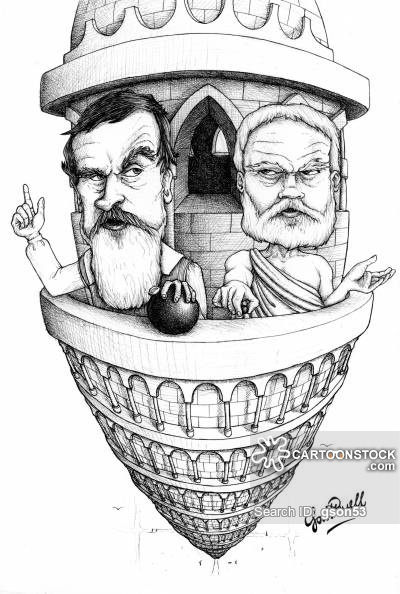
\includegraphics[width=0.8\textwidth]{images/galilei_aristotle_piza.jpg}
                \end{column}
                \begin{column}{0.5\textwidth}
                    \begin{itemize}
                        \item Експерименти с рампи
                        \item $ \Delta v \sim g $
                        \item $ \Delta t \sim 1/g $
                    \end{itemize}
                \end{column}
            \end{columns}
        \end{frame}
    
        \begin{frame}{ Галилеева механика }
            \begin{columns}
                \begin{column}{0.5\textwidth}
                    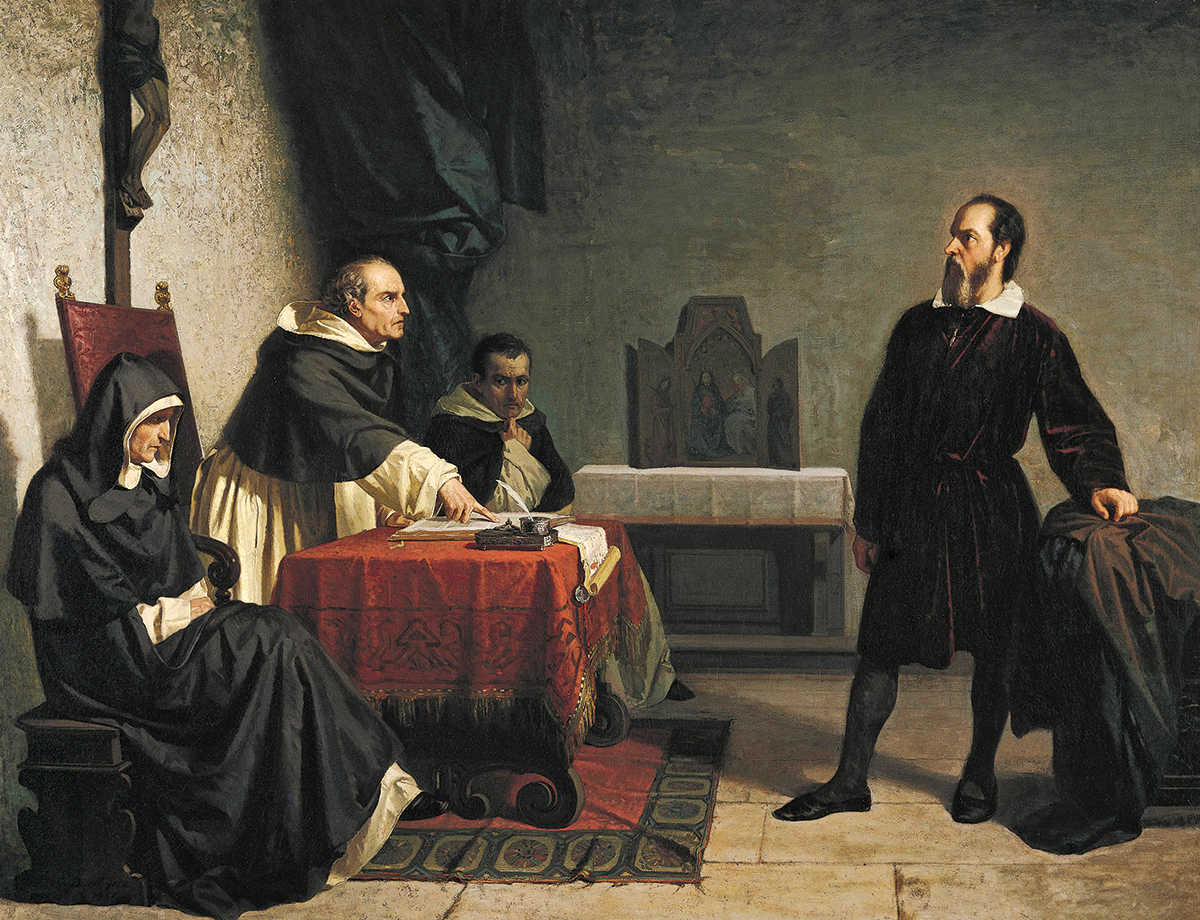
\includegraphics[width=\textwidth]{images/galieli_inqusition.jpg}
                \end{column}
                \begin{column}{0.5\textwidth}
                    \begin{itemize}
                        \item Експерименти с рампи
                        \item $ \Delta v \sim g $
                        \item $ \Delta t \sim 1/g $
                        \item Галилей срещу църквата
                    \end{itemize}
                \end{column}
            \end{columns}
        \end{frame}
        
        \begin{frame}{ Галилеева механика }
            \begin{columns}
                \begin{column}{0.5\textwidth}
                    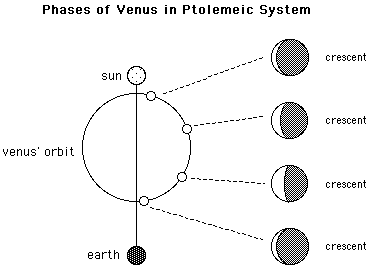
\includegraphics[width=\textwidth]{images/galilei_venus_ptolomey.png}
                \end{column}
            \end{columns}
        \end{frame}
        
        \begin{frame}{ Галилеева механика }
            \begin{columns}
                \begin{column}{0.3\textwidth}
                    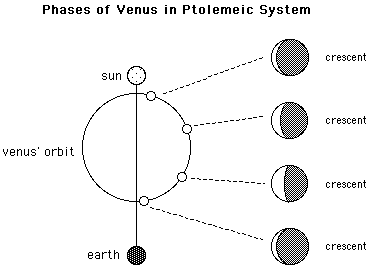
\includegraphics[width=\textwidth]{images/galilei_venus_ptolomey.png}
                \end{column}
                \begin{column}{0.7\textwidth}
                    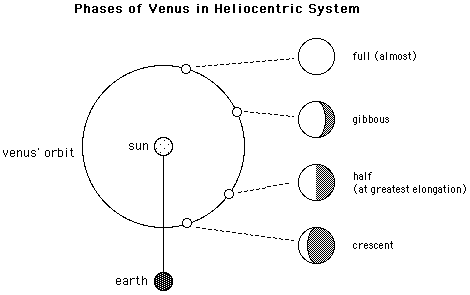
\includegraphics[width=\textwidth]{images/galilei_venus_copernic.png}
                \end{column}
            \end{columns}
        \end{frame}
        
        \begin{frame}{ Галилеева механика }
            \begin{columns}
                \begin{column}{0.5\textwidth}
                    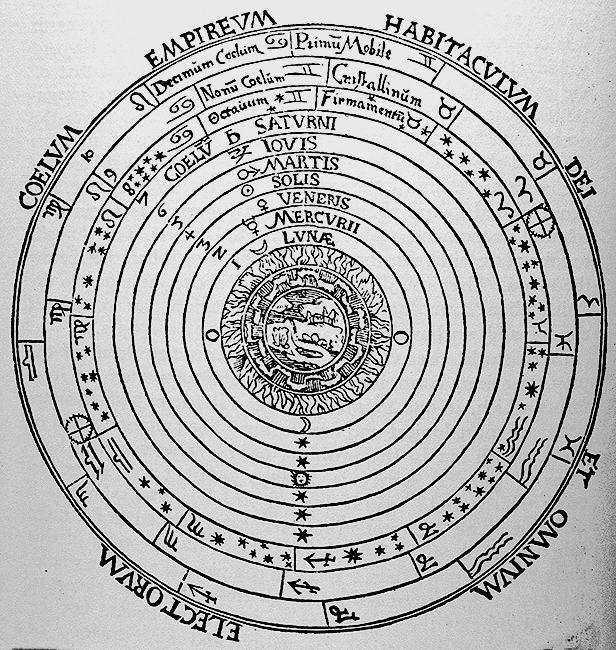
\includegraphics[width=\textwidth]{images/aristotel_universe.png}
                \end{column}
            \end{columns}
        \end{frame}
        
        \begin{frame}{ Галилеева механика }
            \begin{columns}
                \begin{column}{0.2\textwidth}
                    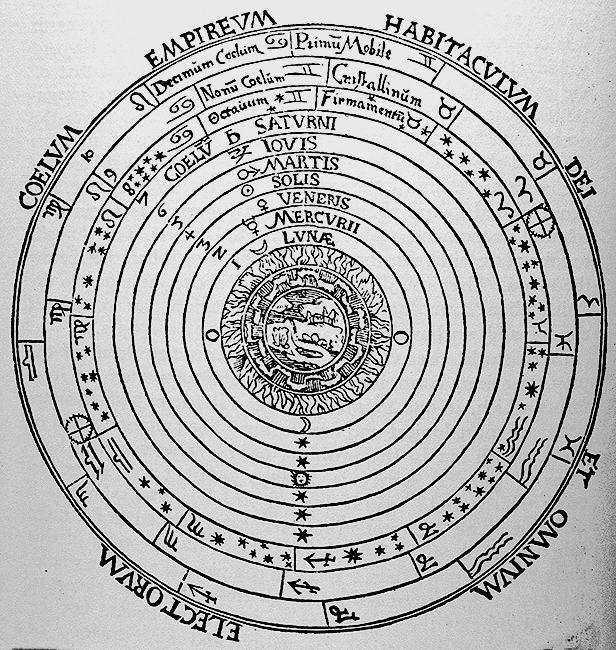
\includegraphics[width=\textwidth]{images/aristotel_universe.png}
                \end{column}
                \begin{column}{0.6\textwidth}
                    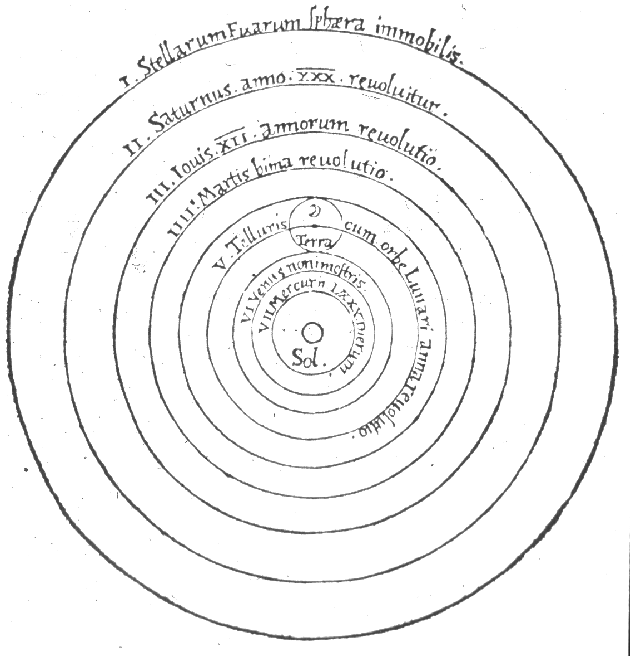
\includegraphics[width=\textwidth]{images/galilei_copernic_model.png}
                \end{column}
            \end{columns}
        \end{frame}
        
        \begin{frame}{ Нютонова механика }
            \begin{columns}
                \begin{column}{0.5\textwidth}
                    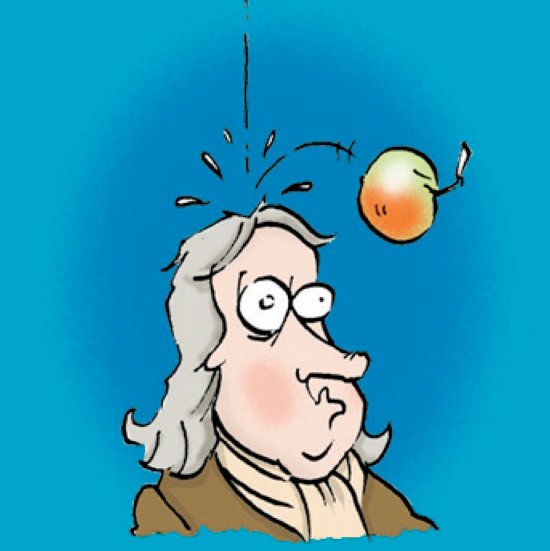
\includegraphics[width=\textwidth]{images/newton_apple.jpg}
                \end{column}
            \end{columns}
        \end{frame}
    
        \begin{frame}{ Нютонова механика }
            \begin{columns}
                \begin{column}{0.5\textwidth}
                    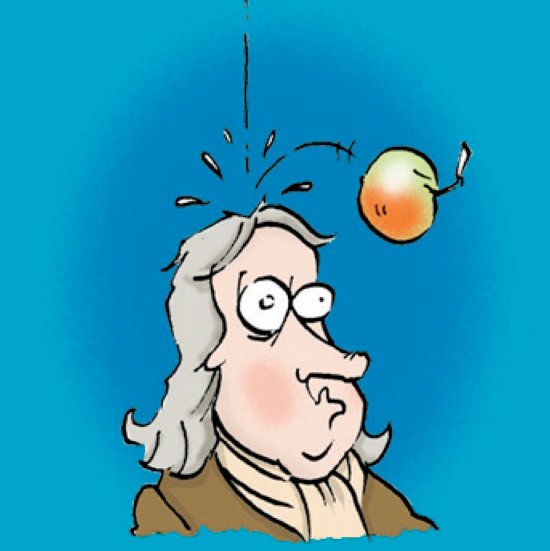
\includegraphics[width=0.9\textwidth]{images/newton_apple.jpg}
                \end{column}
                \begin{column}{0.5\textwidth}
                    \begin{itemize}
                        \item $ F^{\prime} = W - F_{drag} $
                    \end{itemize}
                \end{column}
            \end{columns}
        \end{frame}
        
        \begin{frame}{ Нютонова механика }
            \begin{columns}
                \begin{column}{0.5\textwidth}
                    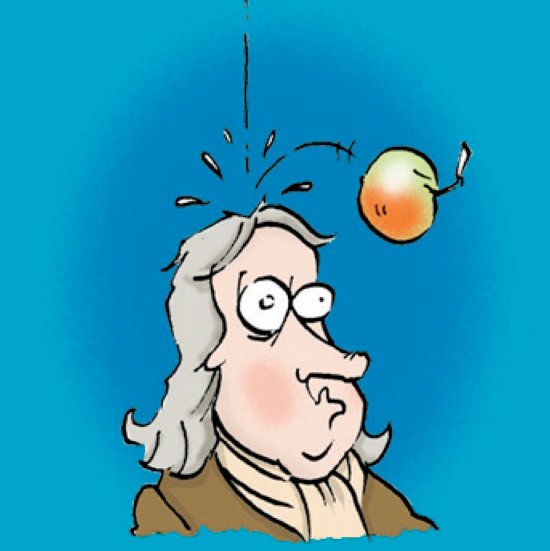
\includegraphics[width=0.9\textwidth]{images/newton_apple.jpg}
                \end{column}
                \begin{column}{0.5\textwidth}
                    \begin{itemize}
                        \item $ F^{\prime} = W - F_{drag} $
                        \item $ g \approx \dfrac{GM}{R^2} = 9.81 \mbox{m/s}^2 $
                    \end{itemize}
                \end{column}
            \end{columns}
        \end{frame}
        
        \begin{frame}{ Нютонова механика }
            \begin{columns}
                \begin{column}{0.5\textwidth}
                    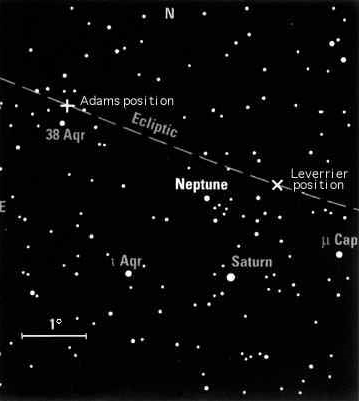
\includegraphics[width=0.9\textwidth]{images/newton_neptune_discovery.png}
                \end{column}
                \begin{column}{0.5\textwidth}
                    \begin{itemize}
                        \item $ F^{\prime} = W - F_{drag} $
                        \item $ g \approx \dfrac{GM}{R^2} = 9.81 \mbox{m/s}^2 $
                        \item Откриване на Нептун, 1946!
                    \end{itemize}
                \end{column}
            \end{columns}
        \end{frame}
    
        \begin{frame}{ Нютонова механика }
            \begin{columns}
                \begin{column}{0.5\textwidth}
                    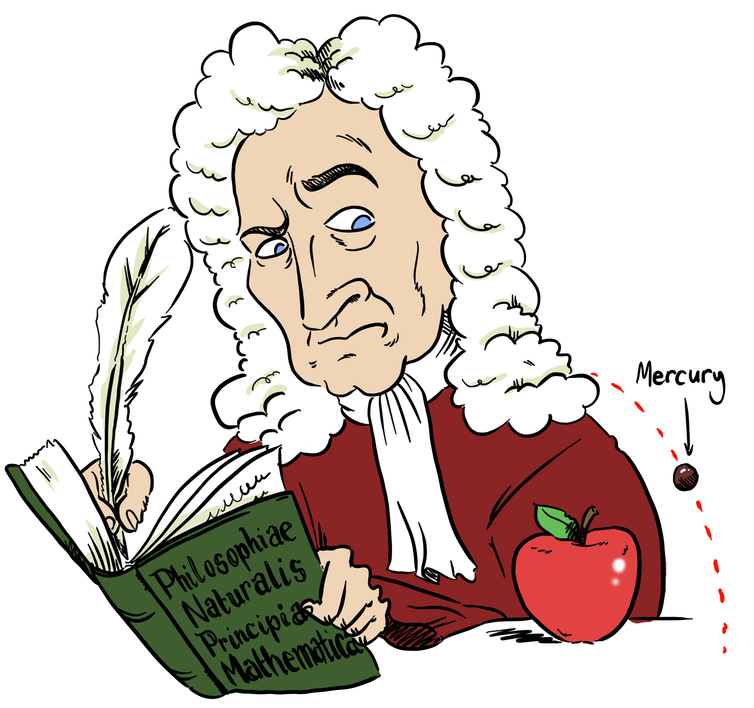
\includegraphics[width=\textwidth]{images/newton_mercury_perih.png}
                \end{column}
            \end{columns}
        \end{frame}
    
        \begin{frame}{ Обща теория на относителността }
            \begin{columns}
                \begin{column}{0.5\textwidth}
                    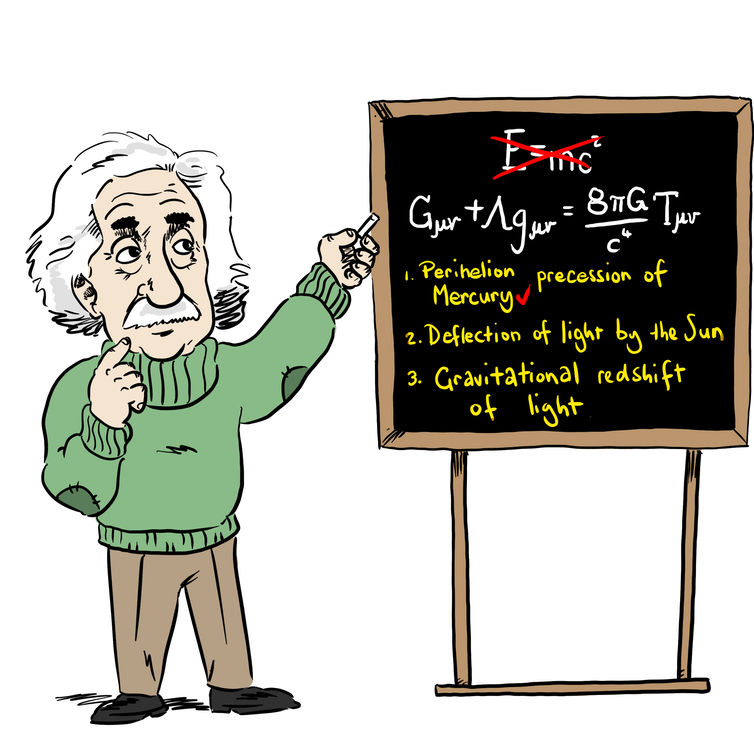
\includegraphics[width=\textwidth]{images/einstein_gr.png}
                \end{column}
            \end{columns}
        \end{frame}
        
    \section{ Настояще }

        \begin{frame}{}
            \tableofcontents[currentsection]
        \end{frame}
        
        \begin{frame}{ Парадокс на Олберт }
            \begin{columns}
                \begin{column}{0.5\textwidth}
                    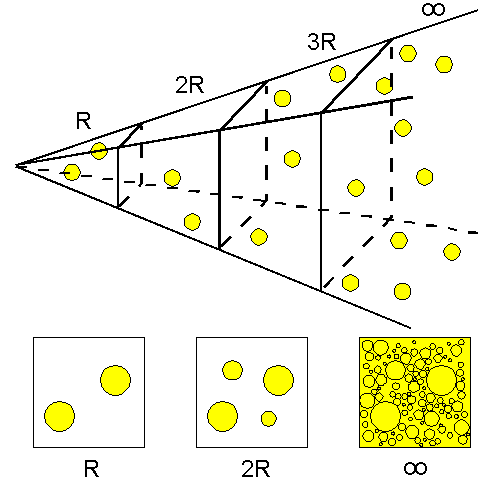
\includegraphics[width=\textwidth]{images/olbers_paradox.png}
                \end{column}
            \end{columns}
        \end{frame}
        
        \begin{frame}{ Парадокс на Олберт }
            \begin{columns}
                \begin{column}{0.5\textwidth}
                    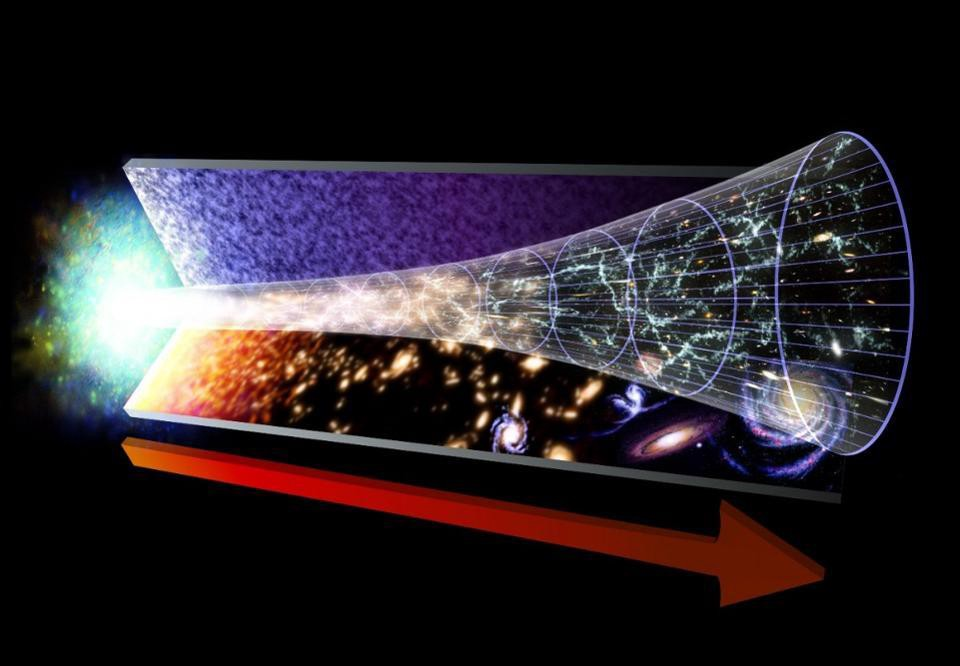
\includegraphics[width=\textwidth]{images/big_bang_theory.jpeg}
                \end{column}
            \end{columns}
        \end{frame}
        
        \begin{frame}{ Парадокс на Олберт }
            \begin{columns}
                \begin{column}{0.5\textwidth}
                    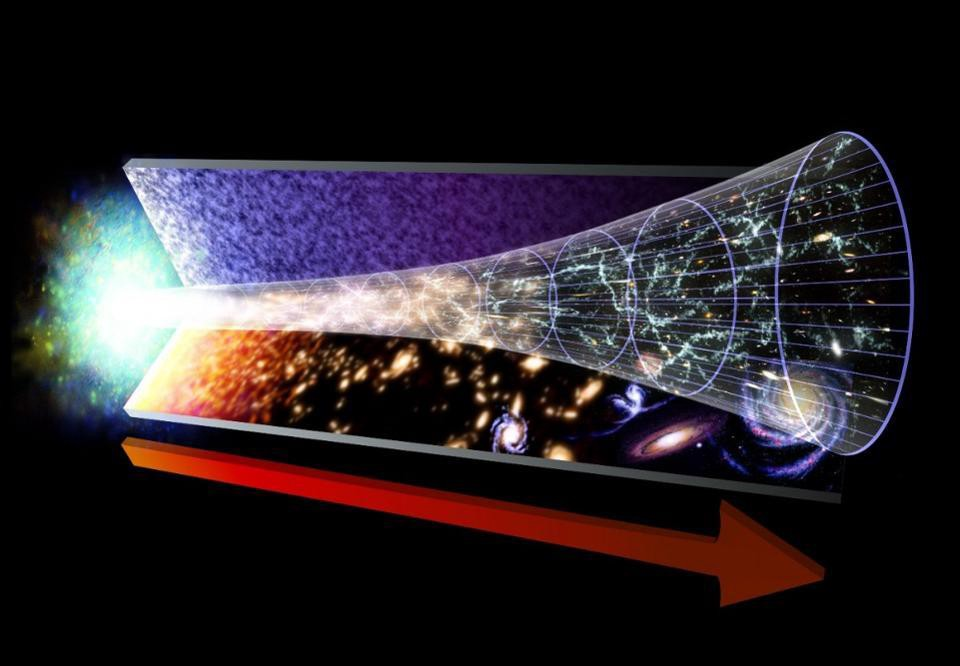
\includegraphics[width=\textwidth]{images/big_bang_theory.jpeg}
                \end{column}
                \begin{column}{0.5\textwidth}
                    \begin{itemize}
                        \item Теория за Големия Взрив \begin{itemize}
                            \item Разширяващата се вселена
                        \end{itemize}
                    \end{itemize}
                \end{column}
            \end{columns}
        \end{frame}
    
        \begin{frame}{ Парадокс на Олберт }
            \begin{columns}
                \begin{column}{0.5\textwidth}
                    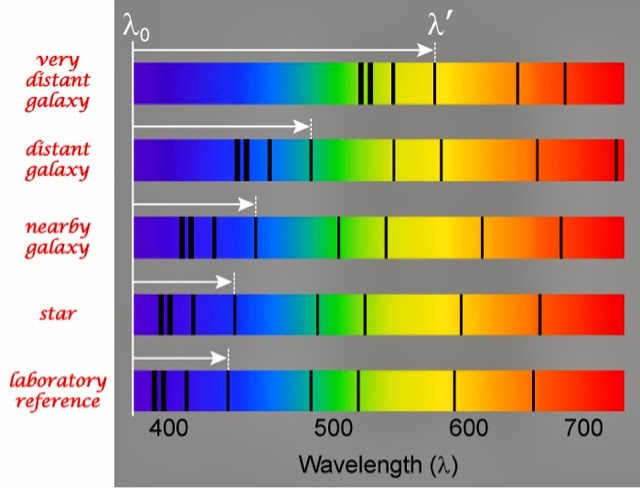
\includegraphics[width=\textwidth]{images/big_bang_redshift.jpg}
                \end{column}
                \begin{column}{0.5\textwidth}
                    \begin{itemize}
                        \item Теория за Големия Взрив \begin{itemize}
                            \item Разширяващата се вселена
                            \item Червено отместване
                        \end{itemize}
                    \end{itemize}
                \end{column}
            \end{columns}
        \end{frame}
        
        \begin{frame}{ Проблеми на ОТО }
            \begin{columns}
                \begin{column}{0.5\textwidth}
                    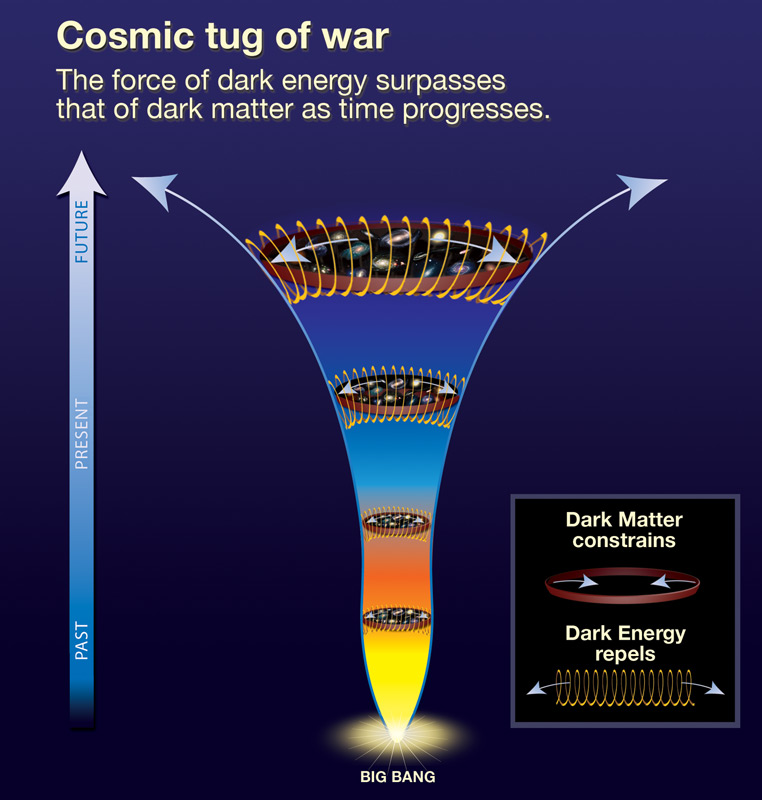
\includegraphics[width=\textwidth]{images/big_bang_acc_expansion.jpg}
                \end{column}
                \begin{column}{0.5\textwidth}
                    \begin{itemize}
                        \item Теория за Големия Взрив \begin{itemize}
                            \item Разширяващата се вселена
                            \item Червено отместване
                            \item Тъмна енергия!!!
                        \end{itemize}
                    \end{itemize}
                \end{column}
            \end{columns}
        \end{frame}
        
        \begin{frame}{ Проблеми на ОТО }
            \begin{columns}
                \begin{column}{0.5\textwidth}
                    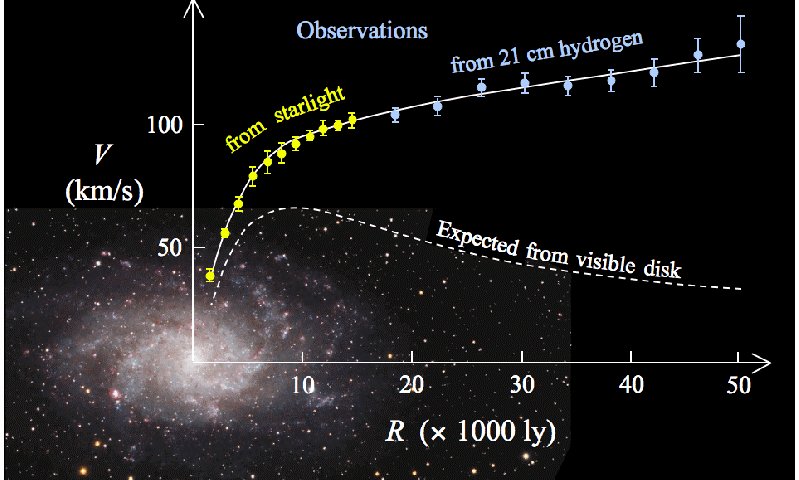
\includegraphics[width=\textwidth]{images/big_bang_dark_matter.png}
                \end{column}
                \begin{column}{0.5\textwidth}
                    \begin{itemize}
                        \item Тъмна енергия!!!
                        \item Тъмна материя!!!
                    \end{itemize}
                \end{column}
            \end{columns}
        \end{frame}
        
    \section{ Бъдеще }
        
        \begin{frame}{ Неутронни звезди }
            
                \begin{columns}
                    \begin{column}{0.8\textwidth}
                            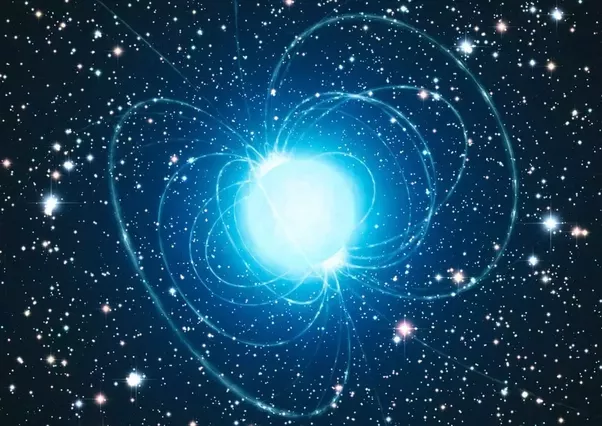
\includegraphics[width=\textwidth]{images/neutron_star.png}
                    \end{column}
                \end{columns}
        \end{frame}
            
        \begin{frame}{ Скаларно-тензорни теории }
            \begin{block}{Общи параметри}
                \begin{itemize}
                    \item куплираща функция $ A(\varphi) $
                    \item сила на полето $ a(\varphi) = \dfrac{dA}{d\varphi} $
                    \item свободен параметър $ \beta = \dfrac{d^2A}{d\varphi^2} $
                    \item потенциал на полето $ V = U(\varphi) $
                \end{itemize}
            \end{block}
        \end{frame}
        
        
	\begin{frame}
		\begin{center}  {\Huge Благодаря за вниманието ! }\end{center}
	\end{frame}
	
\end{document}
